\cptr{How to become a Bayesian in eight easy steps: An annotated reading list}
{How to become a Bayesian in eight easy steps}
{Alexander Etz, Quentin F.\ Gronau, Fabian Dablander, Peter A.\ Edelsbrunner and Beth Baribault}  

\section{Introduction}

In recent decades, significant advances in computational software and hardware have allowed Bayesian statistics to rise to greater prominence in psychology \cite{vandeschoot2016rise}.  In the past few years, this rise has accelerated as a result of increasingly vocal criticism of $p$-values in particular \cite{nickerson2000null,wagenmakers2007practical}, and classical statistics in general \cite{trafimow2015}. When a formerly scarcely used statistical method rapidly becomes more common, editors and peer reviewers are expected to master it readily, and to adequately evaluate and judge manuscripts in which the method is applied. However, many researchers, reviewers, and editors in psychology are still unfamiliar with Bayesian methods.  

We believe that this is at least partly due to the perception that a high level of difficulty is associated with proper use and interpretation of Bayesian statistics. Many seminal texts in Bayesian statistics are dense, mathematically demanding, and assume some background in mathematical statistics \cite<e.g.,>{gelman2014bayesian}.  Even texts that are geared toward psychologists \cite<e.g.,>{LeeWagenmakers2014, Kruschke2015doing}, while less mathematically difficult, require a radically different way of thinking than the classical statistical methods most researchers are familiar with.  Furthermore, transitioning to a Bayesian framework requires a level of time commitment that is not feasible for many researchers.  More approachable sources that survey the core tenets and reasons for using Bayesian methods exist, yet identifying these sources can prove difficult for researchers with little or no previous exposure to Bayesian statistics.  

In this guide, we provide a small number of primary sources that editors, reviewers, and other interested researchers can study to gain a basic understanding of Bayesian statistics.  Each of these sources was selected for their balance of accessibility with coverage of essential Bayesian topics.  By focusing on interpretation, rather than implementation, the guide is able to provide an introduction to core concepts, from Bayes' theorem through to Bayesian cognitive models, without getting mired in secondary details. 

This guide is divided into two primary sections.  The first, \emph{Theoretical sources}, includes commentaries on three articles and one book chapter that explain the core tenets of Bayesian methods as well as their philosophical justification. The second, \emph{Applied sources}, includes commentaries on four articles that cover the most commonly used methods in Bayesian data analysis at a primarily conceptual level. This section emphasizes issues of particular interest to reviewers, such as basic standards for conducting and reporting Bayesian analyses.  

We suggest that for each source, readers first review our commentary, then consult the original source.  The commentaries not only summarize the essential ideas discussed in each source, but also give a sense of how those ideas fit into the bigger picture of Bayesian statistics. This guide is part of a larger special issue in \textit{Psychonomic Bulletin \& Review} on the topic of Bayesian inference that contains articles which elaborate on many of the same points we discuss here, so we will periodically point to these as potential next steps for the interested reader. For those who would like to delve further into the theory and practice of Bayesian methods, the Appendix provides a number of supplemental sources that would be of interest to researchers and reviewers.  To facilitate readers' selection of additional sources, each source is briefly described and has been given a rating by the authors that reflects its level of difficulty and general focus (i.e., theoretical versus applied; see Figure~\ref{fig:8st:scatter}).  It is important to note that our reading list covers sources published up to the time of this writing (August, 2016). 

Overall, the guide is designed such that a researcher might be able to read all eight of the highlighted articles\footnote{Links to freely available versions of each article are provided in the \textit{References} section.} and some supplemental readings within a week.  After readers acquaint themselves with these sources, they should be well-equipped both to interpret existing research and to evaluate new research that relies on Bayesian methods. 

\section{Theoretical sources}
In this section, we discuss the primary ideas underlying Bayesian inference in increasing levels of depth.  Our first source introduces \emph{Bayes' theorem} and demonstrates how Bayesian statistics are based on a different conceptualization of probability than classical, or \textit{frequentist}, statistics \cite{Lindley1993}. These ideas are extended in our second source's discussion of Bayesian inference as a reallocation of credibility between possible states of nature \cite{Kruschke2015doing}.  The third source demonstrates how the concepts established in the previous sources lead to many practical benefits for experimental psychology \cite{Dienes2011}. The section concludes with an in-depth review of Bayesian hypothesis testing using Bayes factors with an emphasis on this technique's theoretical benefits \cite{rouder2009bayesian}. 

\subsection{Conceptual introduction: What is Bayesian inference?} 
\noindent \textbf{Source:} \citeA{Lindley1993} --- The analysis of experimental data: The appreciation of tea and wine
\vspace{2mm}

Lindley leads with a story in which renowned statistician Ronald A.\ Fisher is having his colleague, Dr.\ Muriel Bristol, over for tea. When Fisher prepared the tea---as the story goes---Dr.\ Bristol protested that Fisher had made the tea all wrong. She claims that tea tastes better when milk is added first and infusion second,\footnote{As a historical note:  Distinguishing milk-first from infusion-first tea preparation was not a particular affectation of Dr.\ Bristol's, but a cultural debate that has persisted for over three centuries \cite<e.g.,>{orwell1946nice}.} rather than the other way around; she furthermore professes her ability to tell the difference. Fisher subsequently challenged Dr.\ Bristol to prove her ability to discern the two methods of preparation in a perceptual discrimination study. In Lindley's telling of the story, which takes some liberties with the actual design of the experiment in order to emphasize a point, Dr.\ Bristol correctly identified 5 out of 6 cups where the tea was added either first or second. This result left Fisher faced with the question: Was his colleague merely guessing, or could she really tell the difference? Fisher then proceeded to develop his now classic approach in a sequence of steps, recognizing at various points that tests that seem intuitively appealing actually lead to absurdities, until he arrived at a method that consists of calculating the total probability of the observed result plus the probability of any more extreme results possible under the null hypothesis (i.e., the probability that she would correctly identify 5 \emph{or 6} cups by sheer guessing). This probability is the $p$-value. If it is less than .05, then Fisher would declare the result significant and reject the null hypothesis of guessing.

Lindley's paper essentially continues Fisher's work, showing that Fisher's classic procedure is inadequate and itself leads to absurdities because it hinges upon the nonexistent ability to define what other unobserved results would count as ``more extreme'' than the actual observations. That is, if Fisher had set out to serve Dr. Bristol 6 cups (and only 6 cups) and she is correct 5 times, then we get a $p$-value of .109, which is not statistically significant.  According to Fisher, in this case we should not reject the null hypothesis that Dr.\ Bristol is guessing. But had he set out to keep giving her additional cups until she was correct 5 times, which incidentally required 6 cups, we get a $p$-value of .031, which is statistically significant.  According to Fisher, we should now reject the null hypothesis. Even though the data observed in both cases are exactly the same, we reach different conclusions because our definition of ``more extreme'' results (that did not occur) changes depending on which sampling plan we use. Absurdly, the $p$-value, and with it our conclusion about Dr.\ Bristol's ability, depends on how we think about results that might have occurred but never actually did, and that in turn depends on how we planned the experiment (rather than only on how it turned out).

\begin{figure}[!t]
\centering
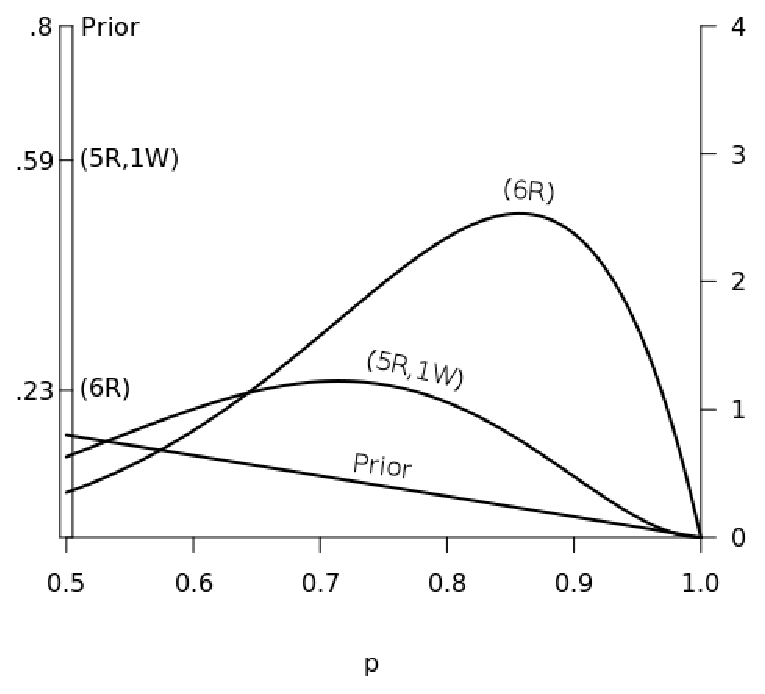
\includegraphics[scale=.9]
{figs/8st_figure1_Lindley1993}
\caption{A reproduction of Figure 2 from Lindley (1993). The left bar indicates the probability that Dr. Bristol is guessing prior to the study (.8), if 5 right and 1 wrong judgments are observed (.59), and if 6 right and 0 wrong judgments are observed (.23). The lines represents Lindley's corresponding beliefs about Dr. Bristol's accuracy if she is not guessing.}
\end{figure}

Lindley's Bayesian solution to this problem considers only the probability of observations actually obtained, avoiding the problem of defining more extreme, unobserved results. The observations are used to assign a probability to each possible value of Dr.\ Bristol's success rate. Lindley's Bayesian approach to evaluating Dr.\ Bristol's ability to discriminate between the differently made teas starts by assigning a priori probabilities across the range of values of her success rate. If it is reasonable to consider that Dr.\ Bristol is simply guessing the outcome at random (i.e., her rate of success is .5), then one must assign an a priori probability to this null hypothesis (see our Figure~1, and note the separate amount of probability assigned to $p=.5$). 
The remaining probability is distributed among the range of other plausible values of Dr.\ Bristol's success rate (i.e., rates that do not assume that she is guessing at random)\footnote{If the null hypothesis is not initially considered tenable, then we can proceed without assigning separate probability to it and instead focus on estimating the parameters of interest (e.g., the taster's accuracy in distinguishing wines, as in Lindley's second example; see Lindley's Figure 1, and notice that the amount of probability assigned to $p=.5$ is gone). Additionally, if a range of values of the parameter is considered impossible---such as rates that are below chance---then this range may be given zero prior probability.}. 
Then the observations are used to update these probabilities using \textit{Bayes' rule} (this is derived in detail in \citeNP{EtzSI}). If the observations fit better with the null hypothesis (pure guessing), then the probability assigned to the null hypothesis will increase; if the data fit better with the alternative hypothesis, then the probability assigned to the alternative hypothesis will increase, and subsequently the probability attached to the null hypothesis will decrease (note the decreasing probability of the null hypothesis on the left axis of Figure~2). The factor by which the data shift the balance of the hypotheses' probabilities is the \textit{Bayes factor} (\citeNP{KassRaftery1995}; see also \citeNP{rouder2009bayesian}, and \citeNP{Dienes2011}, below). 

A key takeaway from this paper is that Lindley's Bayesian approach depends only on the observed data, so the results are interpretable regardless of whether the sampling plan was rigid or flexible or even known at all. Another key point is that the Bayesian approach is inherently \textit{comparative}: Hypotheses are tested against one another and never in isolation. Lindley further concludes that, since the posterior probability that the null is true will often be higher than the $p$-value, the latter metric will discount null hypotheses more easily in general.

\subsection{Bayesian credibility assessments}
\noindent\textbf{Source:} \citeA[Chapter 2]{Kruschke2015doing} --- Introduction: Credibility, models, and parameters

\vspace{2mm}
\begin{quote}
``How often have I said to you that when all other $\theta$ yield $P(x|\theta)$ of $0$, whatever remains, however low its $P(\theta)$, must have $P(\theta|x) = 1$?''
\flushright -- Sherlock Holmes, paraphrased
\end{quote} 
In this book chapter, Kruschke explains the fundamental Bayesian principle of \emph{reallocation of probability}, or ``credibility,'' across possible states of nature. Kruschke uses an example featuring Sherlock Holmes to demonstrate that the famous detective essentially used Bayesian reasoning to solve his cases.
Suppose that Holmes has determined that there exist only four different possible causes (A, B, C, and D) of a committed crime which, for simplicity in the example, he holds to be equally credible at the outset.
This translates to equal \textit{prior} probabilities for each of the four possible causes (i.e., a prior probability of $1/4$ for each).
Now suppose that Holmes gathers evidence that allows him to rule out cause A with certainty.  This development causes the probability assigned to A to drop to zero, and the probability that used to be assigned to cause A to be then redistributed across the other possible causes. Since the probabilities for the four alternatives need to sum to one, the probability for each of the other causes is now equal to $1/3$ (Figure~2.1, p.~17).
What Holmes has done is reallocate credibility across the different possible causes based on the evidence he has gathered.
His new state of knowledge is that only one of the three remaining alternatives can be the cause of the crime and that they are all equally plausible.
Holmes, being a man of great intellect, is eventually able to completely rule out two of the remaining three causes, leaving him with only one possible explanation---which has to be the cause of the crime (as it now must have probability equal to 1), no matter how improbable it might have seemed at the beginning of his investigation.

The reader might object that it is rather unrealistic to assume that data can be gathered that allow a researcher to completely rule out contending hypotheses.
In real applications, psychological data are noisy, and outcomes are only probabilistically linked to the underlying causes.
In terms of reallocation of credibility, this means that possible hypotheses can rarely be ruled out completely (i.e., reduced to zero probability), however, their credibility can be greatly diminished, leading to a substantial increase in the credibility of other possible hypotheses.
Although a hypothesis has not been eliminated, something has been learned: Namely, that one or more of the candidate hypotheses has had their probabilities reduced and are now less likely than the others.

In a statistical context, the possible hypotheses are parameter values in mathematical models that serve to describe the observed data in a useful way.
For example, a scientist could assume that their observations are normally distributed and be interested in which range of values for the mean is most credible. 
Sherlock Holmes only considered a set of discrete possibilities, but in many cases it would be very restrictive to only allow a few alternatives (e.g., when estimating the mean of a normal distribution).
In the Bayesian framework one can easily consider an infinite continuum of possibilities, across which credibility may still be reallocated. It is easy to extend this framework of reallocation of credibility to hypothesis testing situations where one parameter value is seen as ``special'' and receives a high amount of prior probability compared to the alternatives (as in Lindley's tea example above).

\citeA{Kruschke2015doing} serves as a good first introduction to Bayesian thinking, as it requires only basic statistical knowledge (a natural follow-up is \citeNP{KruschkeSI}).  In this chapter, Kruschke also provides a concise introduction to mathematical models and parameters, two core concepts which our other sources will build on.
One final key takeaway from this chapter is the idea of sequential updating from prior to posterior (Figure~2.1, p.~17) as data are collected.
As Dennis Lindley famously said: ``Today’s posterior is tomorrow’s prior'' \cite[p.~2]{Lindley1972}.

\subsection{Implications of Bayesian statistics for experimental psychology}
\noindent\textbf{Source:} \citeA{Dienes2011} --- Bayesian versus orthodox statistics: Which side are you on? 
\vspace{2mm}

Dienes explains several differences between the frequentist (which Dienes calls \textit{orthodox} and we have called \textit{classical}; we use these terms interchangeably) and Bayesian paradigm which have practical implications for how experimental psychologists conduct experiments, analyze data, and interpret results (a natural follow-up to the discussion in this section is available in \citeNP{DienesSI}).
Throughout the paper, Dienes also discusses \textit{subjective} (or context-dependent) Bayesian methods which allow for inclusion of relevant problem-specific knowledge in to the formation of one's statistical model. 

\subsubsection{The probabilities of data given theory and of theory given data}
When testing a theory, both the frequentist and Bayesian approaches use probability theory as the basis for inference, yet in each framework, the interpretation of probability is different.  
It is important to be aware of the implications of this difference in order to correctly interpret frequentist and Bayesian analyses.
One major contrast is a result of the fact that frequentist statistics only allow for statements to be made about $P(\text{data} \mid \text{theory})$\footnote{The conditional probability ($P$) of data given ($\mid$) theory.}: Assuming the theory is correct, the probability of observing the obtained (or more extreme) data is evaluated.
Dienes argues that often the probability of the data assuming a theory is correct is not the probability the researcher is interested in.
What researchers typically want to know is $P(\text{theory} \mid \text{data})$: Given that the data were those obtained, what is the probability that the theory is correct?
At first glance, these two probabilities might appear similar, but Dienes illustrates their fundamental difference with the following example: The probability that a person is dead (i.e., \emph{data}) given that a shark has bitten the person's head off (i.e., \emph{theory}) is 1.
However, given that a person is dead, the probability that a shark has bitten this person's head off is very close to zero \cite<see>[for an intuitive explanation of this distinction]{senn2013invalid}.
It is important to keep in mind that a $p$-value does \emph{not} correspond to $P(\text{theory} \mid \text{data})$; in fact, statements about this probability are only possible if one is willing to attach prior probabilities (degrees of plausibility or credibility) to theories---which can only be done in the Bayesian paradigm.

In the following sections, Dienes explains how the Bayesian approach is more liberating than the frequentist approach with regard to the following concepts: \emph{stopping rules}, \emph{planned versus post hoc comparisons}, and \emph{multiple testing}.
For those new to the Bayesian paradigm, these proposals may seem counterintuitive at first, but Dienes provides clear and accessible explanations for each.
 
\subsubsection{Stopping rules}
In the classical statistical paradigm, it is necessary to specify in advance how the data will be collected. In practice, one usually has to specify how many participants will be collected; stopping data collection early or continuing after the pre-specified number of participants has been reached is not permitted. One reason why collecting additional participants is not permitted in the typical frequentist paradigm is that, given the null hypothesis is true, the $p$-value is not driven in a particular direction as more observations are gathered.  In fact, in many cases the distribution of the $p$-value is uniform when the null hypothesis is true, meaning that every $p$-value is equally likely under the null. 
This implies that even if there is no effect, a researcher is guaranteed to obtain a statistically significant result if they simply continue to collect participants and stop when the $p$-value is sufficiently low. 
In contrast, the Bayes factor, the most common Bayesian method of hypothesis testing, will approach infinite support in favor of the null hypothesis as more observations are collected if the null hypothesis is true. 
Furthermore, since Bayesian inference obeys the \textit{likelihood principle}, one is allowed to continue or stop collecting participants at any time while maintaining the validity of one's results (p.~276; see also \citeNP{cornfield1966}, \citeNP{Rouder2014stopping}, and \citeNP{Royall2004} in the appended \emph{Further Reading} section).

\subsubsection{Planned versus post hoc comparisons}
In the classical hypothesis-testing approach, a distinction is made between planned and post hoc comparisons: It matters whether the hypothesis was formulated before or after data collection. In contrast, Dienes argues that adherence to the likelihood principle entails that a theory does not necessarily need to precede the data when a Bayesian approach is adopted; since this temporal information does not enter into the likelihood function for the data, the evidence for or against the theory will be the same no matter its temporal relation to the data. 

\subsubsection{Multiple testing}
When conducting multiple tests in the classical approach, it is important to correct for the number of tests performed \cite<see>{gelman2014forking}.
Dienes points out that within the Bayesian approach, the number of hypotheses tested does not matter---it is not the number of tests that is important, but the evaluation of how accurately each hypothesis predicts the observed data.
Nevertheless, it is crucial to consider all relevant evidence, including so-called ``outliers,'' because ``cherry picking is wrong on all statistical approaches'' \cite[p.~280]{Dienes2011}. 

\subsubsection{Context-dependent Bayes factors}
The last part of the article addresses how problem-specific knowledge may be incorporated in the calculation of the Bayes factor.
As is also explained in our next highlighted source \cite{rouder2009bayesian}, there are two main schools of Bayesian thought: default (or \textit{objective}) Bayes and context-dependent (or \textit{subjective}) Bayes.
In contrast to the default Bayes factors for general application that are designed to have certain desirable mathematical properties \cite<e.g.,>{Jeffreys1961, rouder2009bayesian, rouder2012regression, rouder2012anova, ly2015jeffreys}, Dienes provides an online calculator\footnote{\url{http://www.lifesci.sussex.ac.uk/home/Zoltan_Dienes/inference/Bayes.htm}} that enables one to obtain context-dependent Bayes factors that incorporate domain knowledge for several commonly used statistical tests. In contrast to the default Bayes factors, which are typically designed to use standardized effect sizes, the context-dependent Bayes factors specify prior distributions in terms of the raw effect size. 
Readers who are especially interested in prior elicitation should see the appendix of Dienes' article for a short review of how to appropriately specify prior distributions that incorporate relevant theoretical information  (and \citeNP{Dienes2014nonsig}, for more details and worked examples).

\subsection{Structure and motivation of Bayes factors}
\noindent \textbf{Source:} \citeA{rouder2009bayesian} --- Bayesian $t$-tests for accepting and rejecting the null hypothesis
\vspace{2mm}

In many cases, a scientist's primary interest is in showing evidence for an \emph{invariance}, rather than a difference. For example, researchers may want to conclude that experimental and control groups do not differ in performance on a task \cite<e.g.,>{vanRavenzwaaij2014}, that participants were performing at chance \cite{dienes2015unconscious}, or that two variables are unrelated \cite{rouder2012regression}. In classical statistics this is generally not possible as significance tests are asymmetric; they can only serve to reject the null hypothesis and never to affirm it. One benefit of Bayesian analysis is that inference is perfectly symmetric, meaning evidence can be obtained that favors the null hypothesis as well as the alternative hypothesis (see \citeNP{Gallistel2009}, as listed in our \emph{Further Reading} appendix). This is made possible by the use of \textit{Bayes factors}.\footnote{Readers for whom Rouder and colleagues' \citeyear{rouder2009bayesian} 
treatment is too technical could focus on Dienes' conceptual ideas and motivations underlying the Bayes factor.} The section covering the shortcomings of classical statistics (``Critiques of Inference by Significance Tests'') can safely be skipped, but readers particularly interested in the motivation of Bayesian inference are advised to read it.

\subsubsection{What is a Bayes factor?}
The Bayes factor is a representation of the relative predictive success of two or more models, and it is a fundamental measure of relative evidence. The way Bayesians quantify predictive success of a model is to calculate the probability of the data given that model---also called the \emph{marginal likelihood} or sometimes simply the \emph{evidence}. The ratio of two such probabilities is the Bayes factor. Rouder and colleagues \citeyear{rouder2009bayesian} denote the probability of the data given some model, represented by $H_i$, as $f(\text{data} \mid H_i)$.\footnote{The probability ($f$) of the observed data given ($\mid$) hypothesis $i$ ($H_i$), where $i$ indicates one of the candidate hypotheses (e.g., 0, 1, A, etc.). The null hypothesis is usually denoted $H_0$ and the alternative hypothesis is usually denoted either $H_1$ or $H_A$.} The Bayes factor for $H_0$ versus $H_1$ is simply the ratio of $f(\text{data} \mid H_0)$ and $f(\text{data} \mid H_1)$ written $B_{01}$ (or $BF_{01}$), where the $B$ (or $BF$) indicates a Bayes factor, and the subscript indicates which two models are being compared (see p.~228). If the result of a study is $B_{01} = 10$ then the data are ten times more probable under $H_0$ than under $H_1$. Researchers should report the exact value of the Bayes factor since it is a continuous measure of evidence, but various benchmarks have been suggested to help researchers interpret Bayes factors, with values between 1 and 3, between 3 and 10, and greater than 10 generally taken to indicate inconclusive, weak, and strong evidence, respectively \cite<see>{Jeffreys1961,wagenmakers2007practical,etzVandekerckhove2016}, although different researchers may set different benchmarks. 
Care is need when interpreting Bayes factors against these benchmarks, as they are not meant to be bright lines against which we judge a study's success (as opposed to how a statistical significance criterion is sometimes treated); the difference between a Bayes factor of, say, 8 and 12 is more a difference of degree than of category. Furthermore, Bayes factors near 1 indicate the data are uninformative, and should not be interpreted as even mild evidence for either of the hypotheses under consideration.  

Readers who are less comfortable with reading mathematical notation may skip over most of the equations without too much loss of clarity. The takeaway is that to evaluate which model is better supported by the data, we need to find out which model has done the best job predicting the data we observe. To a Bayesian, the probability a model assigns to the observed data constitutes its predictive success  \cite<see>{morey2016}; a model that assigns a high probability to the data relative to another model is best supported by the data. The goal is then to find the probability a given model assigns the data, $f(\text{data}\mid H_i)$. Usually the null hypothesis specifies that the true parameter is a particular value of interest (e.g., 0), so we can easily find $f(\text{data}\mid H_0)$. However, we generally do not know the value of the parameter if the null model is false, so we do not know what probability it assigns the data. To represent our uncertainty with regard to the true value of the parameter if the null hypothesis is false, Bayesians specify a range of plausible values that the parameter might take under the alternative hypothesis. All of these parameter values are subsequently used in computing an average probability of the data given the alternative hypothesis, $f(\text{data}\mid H_1)$ (for an intuitive illustration, see \citeNP{Gallistel2009} as listed in our \emph{Further Reading} appendix). If the prior distribution gives substantial weight to parameter values that assign high probability to the data, then the average probability the alternative hypothesis assigns to the data will be relatively high---the model is effectively rewarded for its accurate predictions with a high value for $f(\text{data}\mid H_1)$.

\subsubsection{The role of priors} 
The form of the prior can have important consequences on the resulting Bayes factor. As discussed in our third source \cite{Dienes2011}, there are two primary schools of Bayesian thought: default (objective) Bayes \cite{berger2006} and context-dependent (subjective) Bayes \cite{goldstein2006,rouder2016interplay}. The default Bayesian tries to specify prior distributions that convey little information while maintaining certain desirable properties. For example, one desirable property is that changing the scale of measurement should not change the way the information is represented in the prior, which is accomplished by using standardized effect sizes.
Context-dependent prior distributions are often used because they more accurately encode our prior information about the effects under study, and can be represented with raw or standardized effect sizes, but they do not necessarily have the same desirable mathematical properties (although sometimes they can).

Choosing a prior distribution for the standardized effect size is relatively straightforward for the default Bayesian. One possibility is to use a normal distribution centered at $0$ and with some standard deviation (i.e., spread) $\sigma$. If $\sigma$ is too large, the Bayes factor will always favor the null model, so such a choice would be unwise \cite<see also>{degroot1982lindley,robert2014}. This happens because such a prior distribution assigns weight to very extreme values of the effect size, when in reality, the effect is most often reasonably small (e.g., almost all psychological effects are smaller than Cohen's $d = 2$).
The model is penalized for low predictive success.
Setting $\sigma$ to $1$ is reasonable and common---this is called the \textit{unit information prior}. However, using a Cauchy distribution (which resembles a normal distribution but with less central mass and fatter tails) has some better properties than the unit information prior, and is now a common default prior on the alternative hypothesis, giving rise to what is now called the \textit{default Bayes factor} (see \citeNP{rouder2012regression} for more details; see also \citeNP{LoveSI} and \citeNP{WagenmakersSI}). To use the Cauchy distribution, like the normal distribution, again one must specify a scaling factor. If it is too large, the same problem as before occurs where the null model will always be favored. Rouder and colleagues suggest a scale of 1, which implies that the effect size has a prior probability of 50\% to be between $d = -1$ and $d = 1$. For some areas, such as social psychology, this is not reasonable, and the scale should be reduced. However, slight changes to the scale often do not make much difference in the qualitative conclusions one draws.

Readers are advised to pay close attention to the sections ``Subjectivity in priors'' and ``Bayes factors with small effects.'' The former explains how one can tune the scale of the default prior distribution to reflect more contextually relevant information while maintaining the desirable properties attached to prior distributions of this form, a practice that is a reasonable compromise between the default and context-dependent schools. The latter shows why the Bayes factor will often show evidence in favor of the null hypothesis if the observed effect is small and the prior distribution is relatively diffuse.

\section{Applied sources}

At this point, the essential concepts of Bayesian probability, Bayes' theorem, and the Bayes factor have been discussed in depth.  In the following four sources, these concepts are applied to real data analysis situations. Our first source provides a broad overview of the most common methods of model comparison, including the Bayes factor, with a heavy emphasis on its proper interpretation \cite{vandekerckhove2015model}.  The next source begins by demonstrating Bayesian estimation techniques in the context of developmental research, then provides some guidelines for reporting Bayesian analyses \cite{schoot2014}. Our final two sources discuss issues in Bayesian cognitive modeling, such as the selection of appropriate priors \cite{leeVanpaemel2016}, and the use of cognitive models for theory testing \cite{lee2008}.

Before moving on to our final four highlighted sources, it will be useful if readers consider some differences in perspective among practitioners of Bayesian statistics.  The application of Bayesian methods is very much an active field of study, and as such, the literature contains a multitude of deep, important, and diverse viewpoints on how data analysis should be done, similar to the philosophical divides between Neyman--Pearson and Fisher concerning proper application of classical statistics \cite<see>{lehmann1993fisher}.  The divide between subjective Bayesians, who elect to use priors informed by theory, and objective Bayesians, who instead prefer ``uninformative'' or default priors, has already been mentioned throughout the \textit{Theoretical sources} section above. 

A second division of note exists between Bayesians who see a place for hypothesis testing in science, and those who see statistical inference primarily as a problem of estimation.  The former believe statistical models can stand as useful surrogates for theoretical positions, whose relative merits are subsequently compared using Bayes factors and other such ``scoring'' metrics (as reviewed in \citeNP{vandekerckhove2015model}, discussed below; for additional examples, see \citeNP{Jeffreys1961} and \citeNP{Rouder2016freelunch}). The latter would rather delve deeply into a single model or analysis and use point estimates and credible intervals of parameters as the basis for their theoretical conclusions (as demonstrated in \citeNP{lee2008}, discussed below; for additional examples, see \citeNP{gelman2013philosophy} and \citeNP{mcelreath2016}).\footnote{This divide in Bayesian statistics may be seen as a parallel to the recent discussions about use of classical statistics in psychology \cite<e.g.,>{cumming2014}, where a greater push has been made to adopt an estimation approach over null hypothesis significance testing (NHST). Discussions on the merits of hypothesis testing have been running through all of statistics for over a century, with no end in sight.} 

Novice Bayesians may feel surprised that such wide divisions exist, as statistics (of any persuasion) is often thought of as a set of prescriptive, immutable procedures that can be only right or wrong.  We contend that debates such as these should be expected due to the wide variety of research questions---and diversity of contexts---to which Bayesian methods are applied. As such, we believe that the existence of these divisions speaks to the intellectual vibrancy of the field and its practitioners. We point out these differences here so that readers might use this context to guide their continued reading. 

\subsection{Bayesian model comparison methods}
\noindent\textbf{Source:} \citeA{vandekerckhove2015model} --- Model comparison and the principle of parsimony
\vspace{2mm}

John von Neumann famously said: ``With four parameters I can fit an elephant, and with five I can make him wiggle his trunk'' \cite<as quoted in>[p. 698]{mayer2010}, pointing to the natural tension between model parsimony and goodness of fit. The tension occurs because it is always possible to decrease the amount of error between a model's predictions and the observed data by simply adding more parameters to the model. In the extreme case, any data set of $N$ observations can be reproduced perfectly by a model with $N$ parameters. Such practices, however, termed \emph{overfitting}, result in poor generalization and greatly reduce the accuracy of out-of-sample predictions.
Vandekerckhove and colleagues \citeyear{vandekerckhove2015model} take this issue as a starting point to discuss various criteria for model selection. How do we select a model that both fits the data well and generalizes adequately to new data?

Putting the problem in perspective, the authors discuss research on recognition memory that relies on multinomial processing trees, which are simple, but powerful, cognitive models. Comparing these different models using only the likelihood term is ill-advised, because the model with the highest number of parameters will---all other things being equal---yield the best fit. As a first step to addressing this problem, \citeA{vandekerckhove2015model} discuss the popular Akaike information criterion (AIC) and Bayesian information criterion (BIC).

Though derived from different philosophies \cite<for an overview, see>{aho2014model}, both AIC and BIC try to solve the trade-off between goodness-of-fit and parsimony by combining the likelihood with a penalty for model complexity. However, this penalty is solely a function of the number of parameters and thus neglects the functional form of the model, which can be informative in its own right. As an example, the authors mention Fechner's law and Steven's law. The former is described by a simple logarithmic function, which can only ever fit negatively accelerated data. Steven's law, however, is described by an exponential function, which can account for both positively and negatively accelerated data. Additionally, both models feature just a single parameter, nullifying the benefit of the complexity penalty in each of the two aforementioned information criteria.

The Bayes factor yields a way out. It extends the simple likelihood ratio test by integrating the likelihood with respect to the prior distribution, thus taking the predictive success of the prior distribution into account \cite<see also>[in the \emph{Further Reading} appendix]{Gallistel2009}.
Essentially, the Bayes factor is a likelihood ratio test averaged over all possible parameter values for the model, using the prior distributions as weights: It is the natural extension of the likelihood ratio test to a Bayesian framework. 
The net effect of this is to penalize complex models.  While a complex model can predict a wider range of possible data points than a simple model can, each individual data point is less likely to be observed under the complex model. This is reflected in the prior distribution being more spread out in the complex model.  By weighting the likelihood by the corresponding tiny prior probabilities, the Bayes factor in favor of the complex model decreases. In this way, the Bayes factor instantiates an automatic Ockham's Razor \cite<see also>[in the appended \textit{Further Reading} section]{myung1997}.

However, the Bayes factor can be difficult to compute because it often involves integration over very many dimensions at once.  Vandekerckhove and colleagues \citeyear{vandekerckhove2015model} advocate two methods to ease the computational burden: importance sampling and the Savage-Dickey density ratio (see also \citeNP{wagenmakers2010bayesian} in our in our \textit{Further reading} appendix); additional common computational methods include the Laplace approximation \cite{KassRaftery1995}, bridge sampling \cite{Meng1996bridge,Gronau2017Bridge}, and the encompassing prior approach \cite{hoijtink2008}. They also provide code to estimate parameters in multinomial processing tree models and to compute the Bayes factor to select among them. Overall, the chapter provides a good overview of different methods used to tackle the tension between goodness-of-fit and parsimony in a Bayesian framework. While it is more technical then the sources reviewed above, this article can greatly influence how one thinks about models and methods for selecting among them.

\subsection{Bayesian estimation} 
\noindent\textbf{Source:} \citeA{schoot2014} --- A gentle introduction to Bayesian analysis: Applications to developmental research
\vspace{2mm}

This source approaches practical issues related to parameter estimation in the context of developmental research. This setting offers a good basis for discussing the choice of priors and how those choices influence the posterior estimates for parameters of interest. This is a topic that matters to reviewers and editors alike: How does the choice of prior distributions for focal parameters influence the statistical results and theoretical conclusions that are obtained? The article discusses this issue on a basic and illustrative level.

At this point we feel it is important to note that the difference between hypothesis testing and estimation in the Bayesian framework is much greater than it is in the frequentist framework. In the frequentist framework there is often a one-to-one relationship between the null hypothesis falling outside the sample estimate's 95\% confidence interval and rejection of the null hypothesis with a significance test (e.g., when doing a $t$-test). This is not so in the Bayesian framework; one cannot test a null hypothesis by simply checking if the null value is inside or outside a credible interval. A detailed explanation of the reason for this deserves more space than we can afford to give it here, but in short: When testing hypotheses in the Bayesian framework one should calculate a model comparison metric. See \citeA{RouderSI} for an intuitive introduction to (and synthesis of) the distinction between Bayesian estimation and testing.

Van de Schoot and colleagues \citeyear{schoot2014} begin by reviewing the main differences between frequentist and Bayesian approaches. Most of this part can be skipped by readers who are comfortable with basic terminology at that point. The only newly introduced term is \emph{Markov chain Monte Carlo (MCMC)} methods, which refers to the practice of drawing samples from the posterior distribution instead of deriving the distribution analytically (which may not be feasible for many models; see also \citeNP{vanravenzwaaijSI} and \citeNP{MatzkeSI}). After explaining this alternative approach (p.~848), Bayesian estimation of focal parameters and the specification of prior distributions is discussed with the aid of two case examples.

The first example concerns estimation of an ordinary mean value and the variance of reading scores and serves to illustrate how different sources of information can be used to inform the specification of prior distributions. The authors discuss how expert domain knowledge (e.g., reading scores usually fall within a certain range), statistical considerations (reading scores are normally distributed), and evidence from previous studies (results obtained from samples from similar populations) may be jointly used to define adequate priors for the mean and variance model parameters. The authors perform a prior sensitivity analysis to show how using priors based on different considerations influence the obtained results. Thus, the authors examine and discuss how the posterior distributions of the mean and variance parameters are dependent on the prior distributions used.

The second example focuses on a data set from research on the longitudinal reciprocal associations between personality and relationships. The authors summarize a series of previous studies and discuss how results from these studies may or may not inform prior specifications for the latest obtained data set. Ultimately, strong theoretical considerations are needed to decide whether data sets that were gathered using slightly different age groups can be used to inform inferences about one another.

The authors fit a model with data across two time points and use it to discuss how convergence of the MCMC estimator can be supported and checked.  They then evaluate overall model fit via a posterior predictive check. In this type of model check, data simulated from the specified model are compared to the observed data. If the model is making appropriate predictions, the simulated data and the observed data should appear similar. The article concludes with a brief outline of guidelines for reporting Bayesian analyses and results in a manuscript. Here, the authors emphasize the importance of the specification of prior distributions and of convergence checks (if MCMC sampling is used) and briefly outline how both might be reported. Finally, the authors discuss the use of default priors and various options for conducting Bayesian analyses with common software packages (such as Mplus and WinBUGS).

The examples in the article illustrate different considerations that should be taken into account for choosing prior specifications, the consequences they can have on the obtained results, and how to check whether and how the choice of priors influenced the resulting inferences.

\subsection{Prior elicitation}
\noindent\textbf{Source:} \citeA{leeVanpaemel2016} --- Determining priors for cognitive models
\vspace{2mm}

Statistics does not operate in a vacuum, and often prior knowledge is available that can inform one's inferences. In contrast to classical statistics, Bayesian statistics allows one to formalize and use this prior knowledge for analysis. The paper by \citeA{leeVanpaemel2016} fills an important gap in the literature: What possibilities are there to formalize and uncover prior knowledge?

The authors start by noting a fundamental point: Cognitive modeling \cite<as discussed in our final source,>{lee2008} is an extension of general purpose statistical modeling (e.g., linear regression). Cognitive models are designed to instantiate theory, and thus may need to use richer information and assumptions than general purpose models \cite<see also>{franke2016cogmod}. A consequence of this is that the prior distribution, just like the likelihood, should be seen as an integral part of the model. As \citeA{Jaynes2003ptlos} put it: ``If one fails to specify the prior information, a problem of inference is just as ill-posed as if one had failed to specify the data'' (p.~373). 

What information can we use to specify a prior distribution? Because the parameters in such a cognitive model usually have a direct psychological interpretation, theory may be used to constrain parameter values. For example, a parameter interpreted as a probability of correctly recalling a word must be between 0 and 1. To make this point clear, the authors discuss three cognitive models and show how the parameters instantiate relevant information about psychological processes.  Lee and Vanpaemel also discuss cases in which all of the theoretical content is carried by the prior, while the likelihood does not make any strong assumptions. They also discuss the principle of \textit{transformation invariance}, that is, prior distributions for parameters should be invariant to the scale they are measured on (e.g., measuring reaction time using seconds versus milliseconds). 

Lee and Vanpaemel also discuss specific methods of prior specification. These include the maximum entropy principle, the prior predictive distribution, and hierarchical modeling. The prior predictive distribution is the model-implied distribution of the data, weighted with respect to the prior. Recently, iterated learning methods have been employed to uncover an implicit prior held by a group of participants. These methods can also be used to elicit information that is subsequently formalized as a prior distribution. (For a more in-depth discussion of hierarchical cognitive modeling, see \citeNP{lee2008}, discussed below.)

In sum, the paper gives an excellent overview of why and how one can specify prior distributions for cognitive models. Importantly, priors allow us to integrate domain-specific knowledge, and thus build stronger theories \cite{platt1964strong, Vanpaemel2010}. For more information on specifying prior distributions for data-analytic statistical models rather than cognitive models see \citeA{Rouder2016factorials} and \citeA{Rouder2016anova}.

\subsection{Bayesian cognitive modeling} \noindent\textbf{Source:} \citeA{lee2008} --- Three case studies in the Bayesian analysis of cognitive models
\vspace{2mm}

Our final source \cite{lee2008} further discusses cognitive modeling, a more tailored approach within Bayesian methods. Often in psychology, a researcher will not only expect to observe a particular effect, but will also propose a verbal theory of the cognitive process underlying the expected effect. Cognitive models are used to formalize and test such verbal theories in a precise, quantitative way.  For instance, in a cognitive model, psychological constructs, such as attention and bias, are expressed as model parameters. The proposed psychological process is expressed as dependencies among parameters and observed data (the ``structure'' of the model).

In peer-reviewed work, Bayesian cognitive models are often presented in visual form as a graphical model. Model parameters are designated by nodes, where the shape, shading, and style of border of each node reflect various parameter characteristics.  Dependencies among parameters are depicted as arrows connecting the nodes. Lee gives an exceptionally clear and concise description of how to read graphical models in his discussion of multidimensional scaling \cite[p.~2]{lee2008}.

After a model is constructed, the observed data are used to update the priors and generate a set of posterior distributions. Because cognitive models are typically complex, posterior distributions are almost always obtained through sampling methods (i.e., MCMC; see \citeNP{vanravenzwaaijSI}), rather than through direct, often intractable, analytic calculations. 

Lee demonstrates the construction and use of cognitive models through three case studies. Specifically, he shows how three popular process models may be implemented in a Bayesian framework.  In each case, he begins by explaining the theoretical basis of each model, then demonstrates how the verbal theory may be translated into a full set of prior distributions and likelihoods.  Finally, Lee discusses how results from each model may be interpreted and used for inference.  

Each case example showcases a unique advantage of implementing cognitive models in a Bayesian framework (see also \citeNP{BartlemaSI}). For example, in his discussion of signal detection theory, Lee highlights how Bayesian methods are able to account for individual differences easily \cite<see also>[in the \textit{Further reading} appendix]{rouder2005introduction}. Throughout, Lee emphasizes that Bayesian cognitive models are useful because they allow the researcher to reach new theoretical conclusions that would be difficult to obtain with non-Bayesian methods. Overall, this source not only provides an approachable introduction to Bayesian cognitive models, but also provides an excellent example of good reporting practices for research that employs Bayesian cognitive models.  

\section{Conclusion}
By focusing on interpretation, rather than implementation, we have sought to provide a more accessible introduction to the core concepts and principles of Bayesian analysis than may be found in introductions with a more applied focus.  Ideally, readers who have read through all eight of our highlighted sources, and perhaps some of the supplementary reading, may now feel comfortable with the fundamental ideas in Bayesian data analysis, from basic principles \cite{Kruschke2015doing,Lindley1993} to prior distribution selection \cite{leeVanpaemel2016}, and with the interpretation of a variety of analyses, including Bayesian analogs of classical statistical tests (e.g., $t$-tests; \citeNP{rouder2009bayesian}), estimation in a Bayesian framework \cite{schoot2014}, Bayes factors and other methods for hypothesis testing \cite{Dienes2011,vandekerckhove2015model}, and Bayesian cognitive models \cite{lee2008}. 

Reviewers and editors unfamiliar with Bayesian methods may initially feel hesitant to evaluate empirical articles in which such methods are applied \cite{LoveSI}.  
Ideally, the present article should help ameliorate this apprehension by offering an accessible introduction to Bayesian methods that is focused on interpretation rather than application. Thus, we hope to help minimize the amount of reviewer reticence caused by authors' choice of statistical framework. 

Our overview was not aimed at comparing the advantages and disadvantages of Bayesian and classical methods. However, some conceptual conveniences and analytic strategies that are only possible or valid in the Bayesian framework will have become evident. For example, Bayesian methods allow for the easy implementation of hierarchical models for complex data structures \cite{lee2008}, they allow multiple comparisons and flexible sampling rules during data collection without correction of inferential statistics (\citeNP{Dienes2011}; see also   \citeNP{schonbrodt2015sequential}, as listed in our \textit{Further reading} appendix, and also \citeNP{SchoenbrodtSI}), and they allow inferences that many researchers in psychology are interested in but are not able to answer with classical statistics such as providing support for a null hypothesis (for a discussion, see \citeNP{wagenmakers2007practical}). 
Thus, the inclusion of more research that uses Bayesian methods in the psychological literature should be to the benefit of the entire field \cite{etzVandekerckhove2016}. In this article, we have provided an overview of sources that should allow a novice to understand how Bayesian statistics allow for these benefits, even without prior knowledge of Bayesian methods. 

\section*{Acknowledgments}
The authors would like to thank Jeff Rouder, E.-J. Wagenmakers, and Joachim Vandekerckhove for their helpful comments. AE and BB were supported by grant \#1534472 from NSF's Methods, Measurements, and Statistics panel. AE was further supported by the National Science Foundation Graduate Research Fellowship Program (\#DGE1321846).

\bibliographystyle{apacite}
\bibliography{8st}

\section*{Appendix}

\subsection*{Further reading}

In this Appendix, we provide a concise overview of 32 additional articles and books that provide further discussion of various theoretical and applied topics in Bayesian inference. For example, the list includes articles that editors and reviewers might consult as a reference while reviewing manuscripts that apply advanced Bayesian methods such as structural equation models \cite{kaplan2012bayesian}, hierarchical models \cite{rouder2005introduction}, linear mixed models \cite{sorensen2015hierarchical}, and design (i.e., power) analyses \cite{schonbrodt2015sequential}. The list also includes books that may serve as accessible introductory texts \cite<e.g., >{Dienes2008} or as more advanced textbooks \cite<e.g., >{gelman2014bayesian}.  To aid in readers' selection of sources, we have summarized the associated focus and difficulty ratings for each source in Figure~\ref{fig:8st:scatter}. 

\begin{figure*}[!t]
\centering
  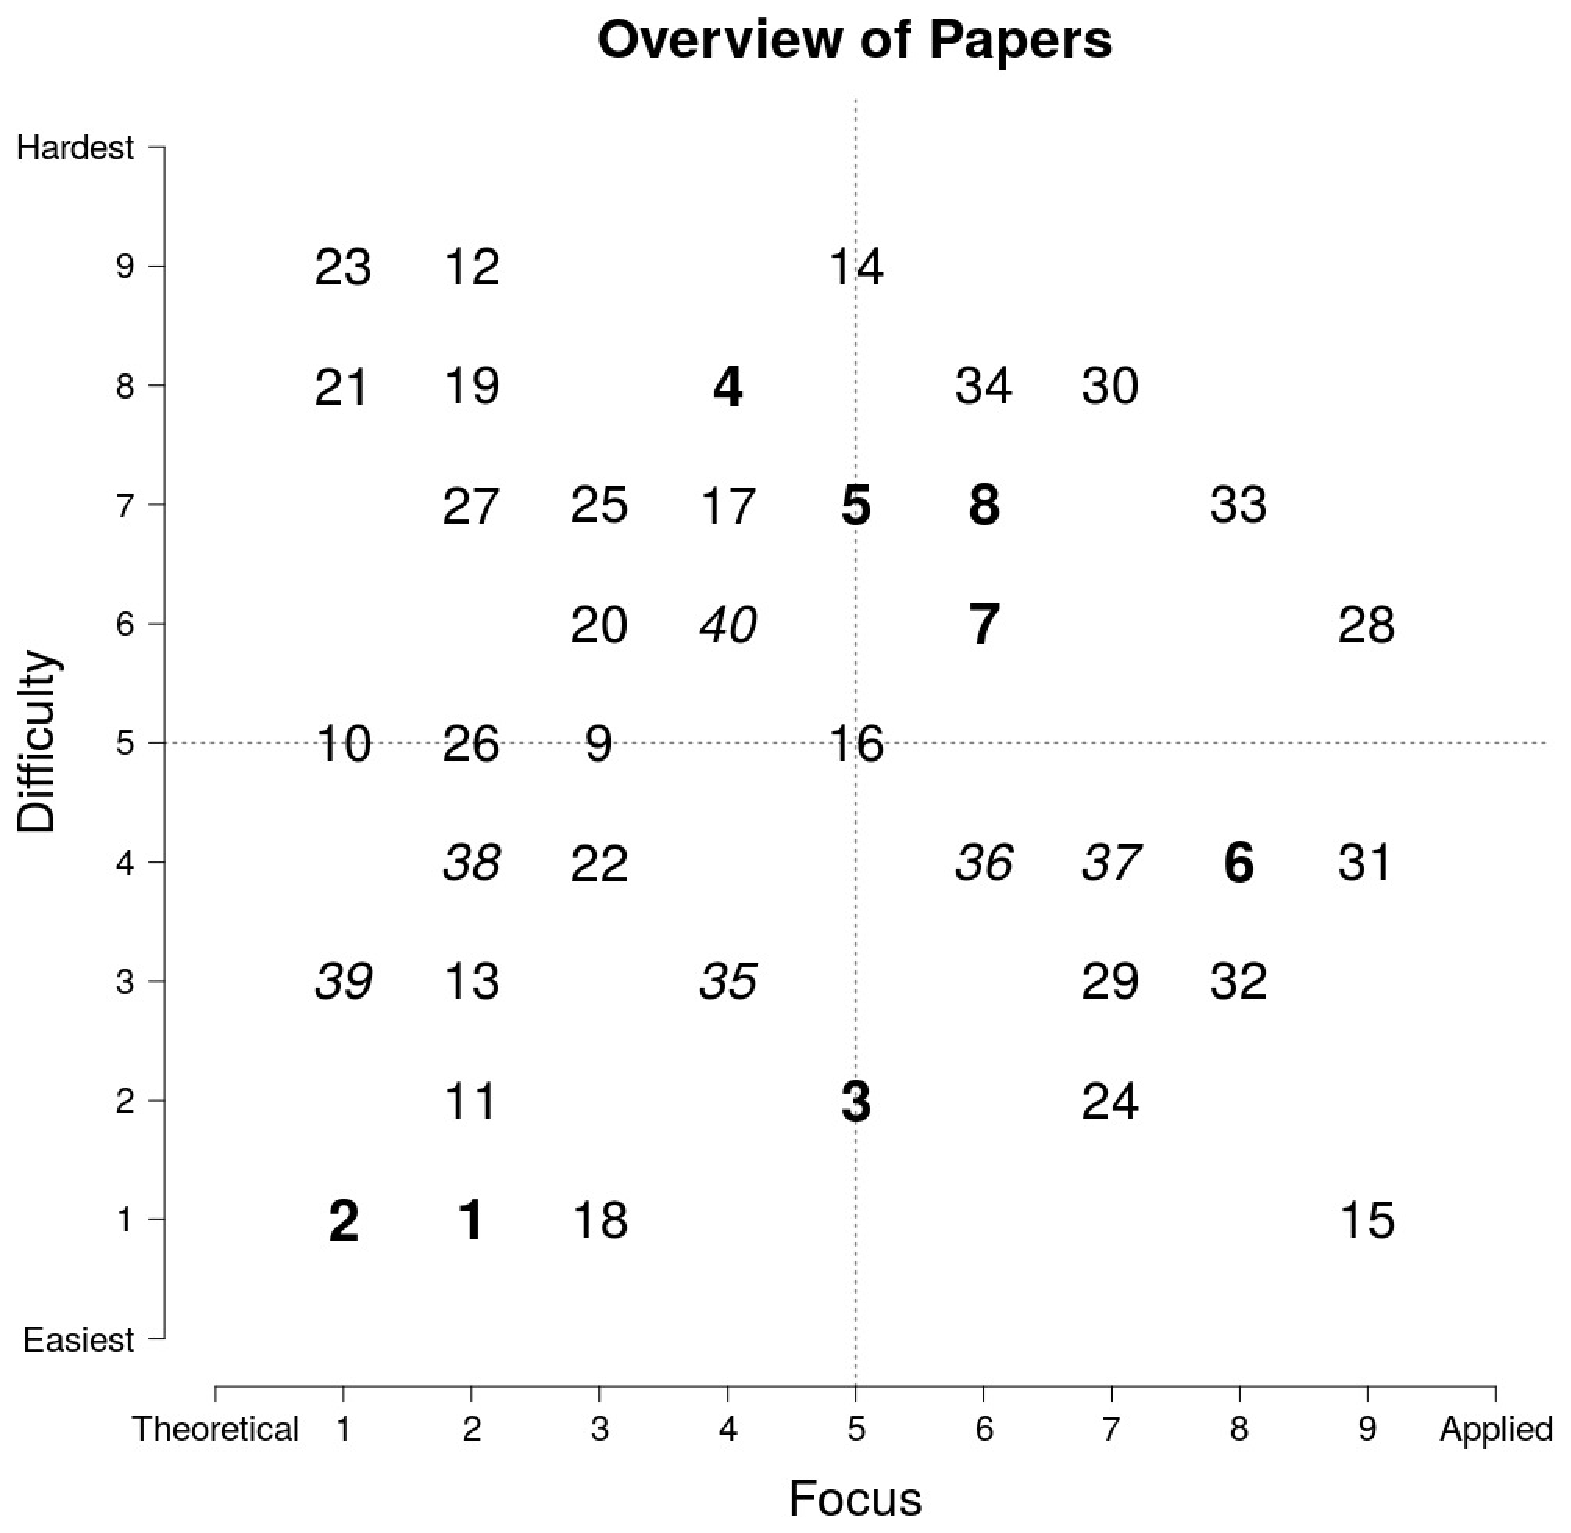
\includegraphics[width=\textwidth]{figs/8st_figureA1_overviewOfPapers}
  \caption{\emph{An overview of focus and difficulty ratings for all sources included in the present paper.}Sources discussed at length in the \emph{Theoretical sources} and \emph{Applied sources} sections are presented in bold text. Sources listed in the appended \emph{Further reading} appendix are presented in light text.  Source numbers representing books are italicized.} 
  \label{fig:8st:scatter}
  
\end{figure*}


\subsection*{Recommended articles}

\begin{enumerate}
  \setcounter{enumi}{8}

\item
\textbf{\citeA{cornfield1966}} --- Sequential Trials, Sequential Analysis, and the Likelihood Principle.  \emph{Theoretical focus (3), moderate difficulty (5).}

A short exposition of the difference between Bayesian and classical inference in sequential sampling problems. 

\item
\textbf{\citeA{lindley2000philosophy}} --- The Philosophy of Statistics.  \emph{Theoretical focus (1), moderate difficulty (5).}

Dennis Lindley, a foundational Bayesian, outlines his philosophy of statistics, receives commentary, and responds. An illuminating paper with equally illuminating commentaries.

\item
\textbf{\citeA{Jaynes1986}} --- Bayesian Methods: General Background.  \emph{Theoretical focus (2), low difficulty (2).}

A brief history of Bayesian inference. The reader can stop after finishing the section titled, ``Is our logic open or closed,'' because the further sections are somewhat dated and not very relevant to psychologists.  

\item
\textbf{\citeA{Edwardsetal1963}} --- Bayesian Statistical Inference for Psychological Research.  \emph{Theoretical focus (2), high difficulty (9).}

The article that first introduced Bayesian inference to psychologists. A challenging but insightful and rewarding paper. Much of the more technical mathematical notation can be skipped with minimal loss of understanding.

\item
\textbf{\citeA{rouder2016interplay}} --- The Interplay between Subjectivity, Statistical Practice, and Psychological Science. \emph{Theoretical focus (2), low difficulty (3)}

All forms of statistical analysis, both Bayesian and frequentist, require some subjective input (see also \citeNP{berger1988}).  In this article, the authors emphasize that subjectivity is in fact desirable, and one of the benefits of the Bayesian approach is that the inclusion of subjective elements is transparent and therefore open to discussion.  

\item \textbf{\citeA{myung1997}} --- Applying Occam's Razor in Cognitive Modeling: A Bayesian Approach.  \emph{Balanced focus (5), high difficulty (9).}

This paper brought Bayesian methods to greater prominence in modern psychology, discussing the allure of Bayesian model comparison for non-nested models and providing worked examples. As the authors provide a great discussion of the principle of parsimony, thus this paper serves as a good follow-up to our fifth highlighted source \cite{vandekerckhove2015model}.

\item \textbf{\citeA{benefits2015wagenmakers}} --- Bayesian Benefits for the Pragmatic Researcher. \emph{Applied focus (9), low difficulty (1).}

Provides pragmatic arguments for the use of Bayesian inference with two examples featuring fictional characters Eric Cartman and Adam Sandler. This paper is clear, witty, and persuasive.

\item
\textbf{\citeA{Rouder2014stopping}} --- Optional Stopping: No Problem for Bayesians. \emph{Balanced focus (5), moderate difficulty (5).}

Provides a simple illustration of why Bayesian inference is valid in the case of optional stopping. A natural follow-up to our third highlighted source \cite{Dienes2011}.

\item  
\textbf{\citeA{verhagen2014bayesian}} --- Bayesian Tests to Quantify the Result of a Replication Attempt. \emph{Balanced focus (4), high difficulty (7).}

Outlines so-called ``replication Bayes factors,'' which use the original study's estimated posterior distribution as a prior distribution for the replication study's Bayes factor. Given the current discussion of how to estimate replicability \cite{open2015estimating}, this work is more relevant than ever. (See also \citeA{wagenmakers2015absence} for a natural follow-up.)

\item
\textbf{\citeA{gigerenzer2004mindless}} --- Mindless Statistics. \emph{Theoretical focus (3), low difficulty (1).}

This paper constructs an enlightening and witty overview on the history and psychology of statistical thinking. It contextualizes the need for Bayesian inference.

\item
\textbf{\citeA{ly2015jeffreys}} --- Harold Jeffreys's Default Bayes Factor Hypothesis Tests: Explanation, Extension, and Application in Psychology. \emph{Theoretical focus (2), high difficulty (8).}

A concise summary of the life, work, and thinking of Harold Jeffreys, inventor of the Bayes factor \cite<see also>{EtzOrigin}. The second part of the paper explains the computations in detail for \textit{t}-tests and correlations. The first part is essential in grasping the motivation behind the Bayes factor.

\item
\textbf{\citeA{robert2014}} --- On the Jeffreys--Lindley Paradox. \emph{Theoretical focus (3), moderate difficulty (6).}

Robert discusses the implications of the Jeffreys--Lindley paradox, so-called because Bayesians and frequentist hypothesis tests can come to diametric conclusions from the same data---even with infinitely large samples. The paper further outlines the need for caution when using \textit{improper priors}, and why they present difficulties for Bayesian hypothesis tests. \cite<For more on this topic see>{degroot1982lindley}.

\item
\textbf{\citeA{jeffreys1936criticisms}} --- On Some Criticisms of the Theory of Probability. \emph{Theoretical focus (1), high difficulty (8).}

An early defense of probability theory's role in scientific inference by one of the founders of Bayesian inference as we know it today. The paper's notation is somewhat outdated and makes for rather slow reading, but Jeffreys's writing is insightful nonetheless.

\item
\textbf{\citeA{Rouder2016freelunch}} --- Is There a Free Lunch in Inference? \emph{Theoretical focus (3), moderate difficulty (4).}

A treatise on why making detailed assumptions about alternatives to the null hypothesis is requisite for a satisfactory method of statistical inference. A good reference for why Bayesians cannot do hypothesis testing by simply checking if a null value lies inside or outside of a credible interval, and instead must calculate a Bayes factor to evaluate the plausibility of a null model.

\item
\textbf{\citeA{berger1987testing}} --- Testing Precise Hypotheses. \emph{Theoretical focus (1), high difficulty (9).}

Explores the different conclusions to be drawn from hypothesis tests in the classical versus Bayesian frameworks. This is a resource for readers with more advanced statistical training.

\item
\textbf{\citeA{wetzels2011statistical}} --- Statistical Evidence in Experimental Psychology: An Empirical Comparison using 855 $t$-tests. \emph{Applied focus (7), low difficulty (2).}

Using 855 $t$-tests from the literature, the authors quantify how inference based on $p$ values, effect sizes, and Bayes factors differ. An illuminating reference to understand the practical differences between various methods of inference.

\item
\textbf{\citeA{Vanpaemel2010}} --- Prior Sensitivity in Theory Testing: An Apologia for the Bayes Factor. \emph{Theoretical focus (3), high difficulty (7).}

The authors defend Bayes factors against the common criticism that the inference is sensitive to specification of the prior.  They assert that this sensitivity is valuable and desirable.

\item
\textbf{\citeA{Royall2004}} --- The Likelihood Paradigm for Statistical Inference. \emph{Theoretical focus (2), moderate difficulty (5).}

An accessible introduction to the Likelihood principle, and its relevance to inference. Contrasts are made among different accounts of statistical evidence. A more complete account is given in \citeA{Royall1997}.

\item
\textbf{\citeA{gelman2013philosophy}} --- Philosophy and the Practice of Bayesian Statistics. \emph{Theoretical focus (2), high difficulty (7).}

This is the centerpiece of an excellent special issue on the philosophy of Bayesian inference. We recommend that discussion groups consider reading the entire special issue (\textit{British Journal of Mathematical and Statistical Psychology}, February, 2013), as it promises intriguing and fundamental discussions about the nature of inference.

\item \textbf{\citeA{wagenmakers2010bayesian}} --- Bayesian Hypothesis Testing for Psychologists: A Tutorial on the Savage-Dickey Ratio. \emph{Applied focus (9), moderate difficulty (6).}

Bayes factors are notoriously hard to calculate for many types of models. This article introduces a useful computational trick known as the ``Savage-Dickey Density Ratio,'' an alternative conception of the Bayes factor that makes many computations more convenient. The Savage-Dickey ratio is a powerful visualization of the Bayes factor, and is the primary graphical output of the Bayesian statistics software JASP \cite{JASP2015}.

\item
\textbf{\citeA{Gallistel2009}} --- The Importance of Proving the Null. \emph{Applied focus (7), low difficulty (3).}

The importance of null hypotheses is explored through three thoroughly worked examples. This paper provides valuable guidance for how one should approach a situation in which it is theoretically desirable to accumulate evidence for a null hypothesis.

\item \textbf{\citeA{rouder2005introduction}} --- An Introduction to Bayesian Hierarchical Models with an Application in the Theory of Signal Detection. \emph{Applied focus (7), high difficulty (8).}

This is a good introduction to hierarchical Bayesian inference for the more mathematically inclined readers. It demonstrates the flexibility of hierarchical Bayesian inference applied to signal detection theory, while also introducing augmented Gibbs sampling.

\item \textbf{\citeA{sorensen2015hierarchical}} --- Bayesian Linear Mixed Models Using Stan: A Tutorial for Psychologists. \emph{Applied focus (9), moderate difficulty (4).}

Using the software Stan, the authors give an accessible and clear introduction to hierarchical linear modeling. Because both the paper and code are hosted on github, this article serves as a good example of open, reproducible research in a Bayesian framework.

\item \textbf{\citeA{schonbrodt2015sequential}} --- Sequential Hypothesis Testing with Bayes Factors: Efficiently Testing Mean Differences. \emph{Applied focus (8), low difficulty (3).}

For Bayesians, power analysis is often an afterthought because sequential sampling is encouraged, flexible, and convenient. This paper provides Bayes factor simulations that give researchers an idea of how many participants they might need to collect to achieve moderate levels of evidence from their studies. 

\item \textbf{\citeA{kaplan2012bayesian}} --- Bayesian Structural Equation Modeling. \emph{Applied focus (8), high difficulty (7).}

One of few available practical sources on Bayesian structural equation modeling. The article focuses on the Mplus software but also stands a general source.

\item \textbf{\citeA{Rouder2016factorials}} --- Bayesian Analysis of Factorial Designs. \emph{Balanced focus (6), high difficulty (8).}

Includes examples of how to set up Bayesian ANOVA models, which are some of the more challenging Bayesian analyses to perform and report, as intuitive hierarchical models. In the appendix, how to use the BayesFactor R package and JASP software for ANOVA is demonstrated. The relatively high difficulty rating is due to the large amount of statistical notation.

\end{enumerate}

\subsection*{Recommended books}

\begin{enumerate}
  \setcounter{enumi}{34}

\item 
\textbf{\citeA{winkler2003}} --- Introduction to Bayesian Inference and Decision. \textit{Balanced focus (4), low difficulty (3).}

As the title suggests, this is an accessible textbook that introduces the basic concepts and theory underlying the Bayesian framework for both inference and decision-making. The required math background is elementary algebra (i.e., no calculus is required).

\item
\textbf{\citeA{mcelreath2016}} --- Statistical Rethinking: A Bayesian Course with Examples in R and Stan. \textit{Balanced focus (6), moderate difficulty (4).}

Not your traditional applied introductory statistics textbook. McElreath focuses on education through simulation, with handy R code embedded throughout the text to give readers a hands-on experience. 

\item
\textbf{\citeA{LeeWagenmakers2014}} --- Bayesian Cognitive Modeling: A Practical Course. \emph{Applied focus (7), moderate difficulty (4).}

A textbook on Bayesian cognitive modeling methods that is in a similar vein to our eighth highlighted source \cite{lee2008}. It includes friendly introductions to core principles of implementation and many case examples with accompanying MATLAB and R code. 

\item
\textbf{\citeA{lindley2006understanding}} --- Understanding Uncertainty. \emph{Theoretical focus (2), moderate difficulty (4).}

An introduction to thinking about uncertainty and how it influences everyday life and science. Lindley proposes that all types of uncertainty can be represented by probabilities. A largely non-technical text, but a clear and concise introduction to the general Bayesian perspective on decision making under uncertainty. 

\item
\textbf{\citeA{Dienes2008}} --- Understanding Psychology as a Science: An Introduction to Scientific and Statistical Inference. \emph{Theoretical focus (1), low difficulty (3).}

A book that covers a mix of philosophy of science, psychology, and Bayesian inference. It is a very accessible introduction to Bayesian statistics, and it very clearly contrasts the different goals of Bayesian and classical inference. 

\item
\textbf{\citeA{Stone2013bayes}} --- Bayes' Rule: A Tutorial Introduction to Bayesian Analysis. \emph{Balanced focus (4), moderate difficulty (6).}

In this short and clear introductory text, Stone explains Bayesian inference using accessible examples and writes for readers with little mathematical background. Accompanying Python and MATLAB code is provided on the author's website.



\end{enumerate}
